\newcounter{nuserstory}
\newcounter{nusecase}

\newcommand{\userstory}[4]{%
    \refstepcounter{nuserstory}
    \subsection{#1}
    \label{userstory:\thenuserstory}
    \hangindent=40pt
    \textbf{\textit{As a}} #2,\\
    \textbf{\textit{I want to}} #3,\\
    \textbf{\textit{so that}} #4.
}
\newenvironment{usecase}[1]
{
    \refstepcounter{nusecase}%
    \subsection{Use Case \thenusecase: #1}%
    \label{usecase:\thenusecase}%
}{}

% With user stories (\userstory) you can reference them back later with \ref{userstory:n}
% For example, first user story in this file can be referred with \ref{userstory:1}

\chapter{Requirement Analysis}
\label{chap:requirement-analysis}

\section{Stakeholder Analysis}
\label{section:stakeholder-analysis}

\subsection{Primary Stakeholders}
\label{subsection:primary-stakeholders}

\begin{enumerate}[leftmargin=80pt]
    \item \textbf{Users:} The primary stakeholders are the users of our multi-camera tracking system, including security personnel, facility managers, emergency response coordinators, and research analysts.  Their interaction with the system is crucial for effective monitoring, incident response, and data-driven decision-making.  For a detailed specification of our users, see \ref{section:target-user}.
    \item \textbf{System Administrators:}  These individuals are responsible for the installation, configuration, and maintenance of the system.  Their needs include ease of deployment, system stability, and access to diagnostic tools.
    \item \textbf{University/Factory Management:}  These stakeholders are interested in the overall benefits of the system, such as improved safety, optimized resource allocation, and enhanced operational efficiency.  They require reports and data summaries to justify the investment and track performance.
    \item \textbf{MTMMC Dataset Providers/Owners:} The creators and distributors of the Multi-Target Multi-Camera (MTMMC) dataset used for training and evaluating the AI components of this project (\ref{subsection:dataset-information}).
        \begin{itemize}
            \item \textbf{Stake:} They have an interest in ensuring the dataset is used responsibly and ethically, strictly according to the terms and conditions outlined in the usage agreement signed by the project team. This includes preventing misuse or unauthorized redistribution of the data.
            \item \textbf{Project Consideration:} The project must adhere to all stipulations in the dataset usage license. Compliance will be documented, and proper attribution/citation will be provided in all relevant project outputs.
        \end{itemize}
\end{enumerate}

\section{User Stories}
\label{section:user-stories}

%% User Stories Start

\userstory{Continuously Track Individuals Across the Area%
}{security officer%
}{continuously track individuals as they move throughout the monitored area, even when they move between different camera views%
}{I can maintain uninterrupted surveillance of persons of interest and respond quickly to developing situations.}

\userstory{Maintain Tracking During Brief Disappearances%
}{security officer%
}{maintain the track of individuals even if they are temporarily out of sight of all cameras%
}{I can have a complete picture of a person's movements, even if they briefly go around corners or into areas without direct camera coverage.}

\userstory{Visualize Movement Paths%
}{facility manager%
}{see a visual representation of how people move through the facility, including their paths and locations over time%
}{I can understand space usage, identify congestion points, and make informed decisions about facility layout and resource allocation.}

\userstory{Access Historical Movement Data%
}{analytics specialist%
}{access and analyze historical data on individual and group movements, including options to export this data%
}{I can perform in-depth analysis of movement patterns, identify trends, and generate reports to improve operational efficiency and space utilization.  I can also share this data with other systems.}

\userstory{Prioritize Tracking of Specific Individuals%
}{security officer/emergency coordinator%
}{designate specific individuals for increased monitoring and receive immediate updates on their location%
}{I can focus on persons of interest during security incidents or emergencies, ensuring a rapid and effective response.}

\userstory{Ensure System Reliability and Uptime%
}{system administrator%
}{easily monitor system performance, troubleshoot issues, and perform necessary maintenance tasks%
}{I can keep the tracking system running smoothly and minimize disruptions to users.}
%% User Stories End

\section{Use Case Diagram}
\label{section:use-case-diagram}

\begin{figure}[h!]
    \centering
    \begin{tikzpicture}

        % System boundary
        \begin{umlsystem}[x=4]{SpotOn}
            % Use cases inside the system boundary
            \umlusecase[name=track, y=4, width=3cm]{Track Individual Across Cameras}
            \umlusecase[name=maintain, y=1.5, width=4cm]{Maintain Tracking During Temporary Disappearance}
            \umlusecase[name=visualize, y=-1, width=3.5cm]{Visualize Movement Paths on a Map}
            \umlusecase[name=prioritize, y=-3.5, width=4cm]{Prioritize Tracking of Specific Individual}
        \end{umlsystem}

        % Actors outside the system boundary
        \umlactor[x=-4, y=3]{Security Officer}
        \umlactor[x=-4, y=0]{Facility Manager}
        \umlactor[x=-4, y=-2]{Analytics Specialist}
        \umlactor[x=-4, y=-4]{Emergency Coordinator}

        % Associations between actors and use cases
        % Security Officer associations
        \umlassoc{Security Officer}{track}
        \umlassoc{Security Officer}{maintain}
        \umlassoc{Security Officer}{prioritize}

        % Facility Manager association
        \umlassoc{Facility Manager}{visualize}

        % Analytics Specialist association
        \umlassoc{Analytics Specialist}{visualize}

        % Emergency Coordinator association
        \umlassoc{Emergency Coordinator}{prioritize}

    \end{tikzpicture}
    \caption{Use Case Diagram of SpotOn Multi-Camera Tracking System}
    \label{fig:use-case-diagram}
\end{figure}
\clearpage
The use case diagram (Figure \ref{fig:use-case-diagram}) illustrates the interactions between different user roles (actors) and the core functionalities (use cases) of the SpotOn Multi-Camera Tracking System. The actors, shown on the left side of the diagram, represent the primary user groups interacting with the system:

\begin{itemize}
    \item \textbf{Security Officer:} Interacts with tracking, maintaining tracking through gaps, and prioritizing specific individuals.
    \item \textbf{Facility Manager:} Primarily interacts with visualizing movement paths.
    \item \textbf{Analytics Specialist:} Also interacts with visualizing movement paths for analysis.
    \item \textbf{Emergency Coordinator:} Interacts with prioritizing the tracking of specific individuals during critical events.
\end{itemize}
This diagram provides a high-level overview of who uses the system and for what main purposes.

\section{Use Case Model}
\label{section:use-case-model}

\begin{usecase}{Track Individual Across Cameras}
    \textbf{Actors:} Security Officer

    \textbf{Description:} Track an individual's movements across multiple camera views.

    \textbf{Scenario:}
    \begin{enumerate}[leftmargin=80pt]
        \item Log into SpotOn.
        \item Select a location and date.
        \item View available camera feeds.
        \item See people with assigned IDs in each camera view.
        \item View a map showing detected individuals.
        \item Select an individual in any camera view.
        \item See that individual highlighted in all cameras where they appear.
        \item View their movement history on the map.
    \end{enumerate}
\end{usecase}

\begin{usecase}{Maintain Tracking During Temporary Disappearance}
    \textbf{Actors:} Security Officer

    \textbf{Description:} Continue tracking an individual even when temporarily out of camera view.

    \textbf{Scenario:}
    \begin{enumerate}[leftmargin=80pt]
        \item Track an individual in the system.
        \item When the person moves out of all camera views, the system marks this state.
        \item When the person reappears, the system reconnects their identity.
        \item See the individual's complete path, with estimated routes during gaps shown as dashed lines.
    \end{enumerate}
\end{usecase}

\begin{usecase}{Visualize Movement Paths on a Map}
    \textbf{Actors:} Facility Manager/Analytics Specialist

    \textbf{Description:} View movement patterns within a facility for space utilization analysis.

    \textbf{Scenario:}
    \begin{enumerate}[leftmargin=80pt]
        \item Log into SpotOn.
        \item Select a location and date.
        \item View a bird's-eye map of the facility.
        \item See movement paths of all individuals overlaid on the map.
        \item Filter paths by camera view.
        \item Select an individual to highlight only their path.
    \end{enumerate}
\end{usecase}

\begin{usecase}{Prioritize Tracking of Specific Individual}
    \textbf{Actors:} Security Officer/Emergency Coordinator

    \textbf{Description:} Focus system resources on tracking a specific individual.

    \textbf{Scenario:}
    \begin{enumerate}[leftmargin=80pt]
        \item Log into SpotOn.
        \item Select a location and date.
        \item View camera feeds and detected individuals.
        \item Designate an individual for prioritized tracking.
        \item See visual highlighting of the prioritized individual in all cameras.
        \item View their position, detection time, tracking duration, and movement details.
    \end{enumerate}
\end{usecase}

% Use Cases End
% \newpage

\section{User Interface Design}
\label{section:user-interface-design}

The user interface for the multi-camera tracking system is designed to offer a clear, intuitive, and efficient experience for security personnel, facility managers, and other stakeholders, focusing on retrospective analysis of recorded video feeds.  The interface prioritizes the visualization of movement patterns, easy access to detailed tracking information.
% Mockup Start

\begin{figure}[h!]
    \centering
    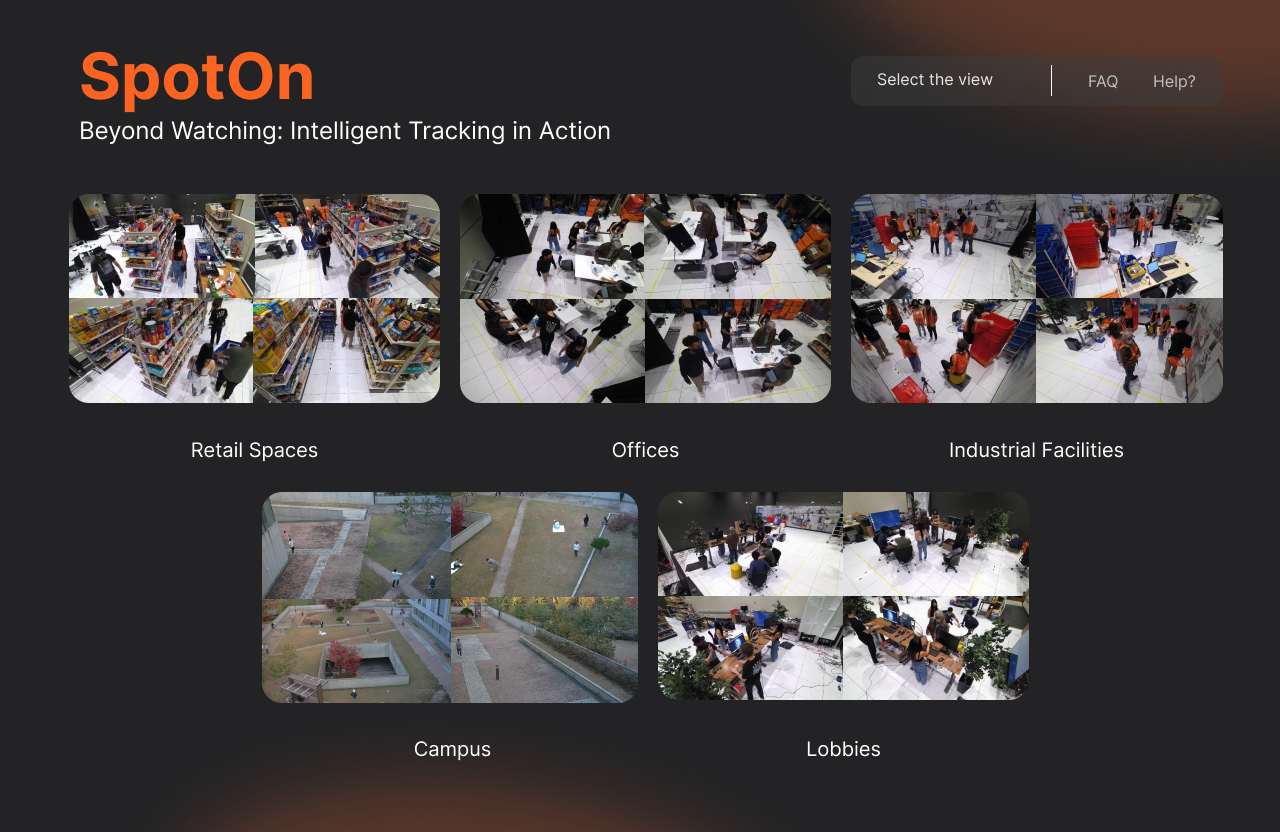
\includegraphics[width=0.8\textwidth,keepaspectratio]{jubjones/mockup/Dashboard.png}
    \caption{Mockup of Landing Page}
    \label{fig:mockup-landing-page}
\end{figure}

\begin{figure}[h!]
    \centering
    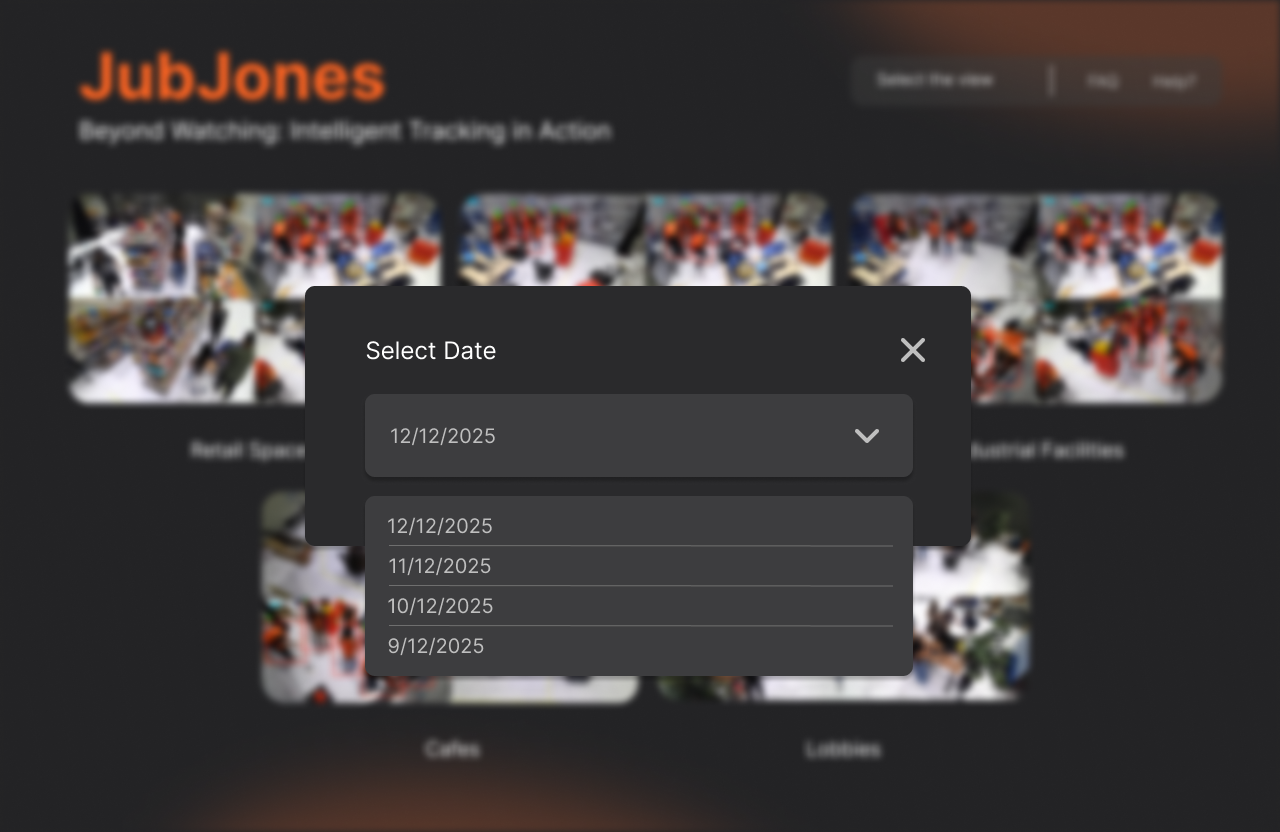
\includegraphics[width=0.8\textwidth,keepaspectratio]{jubjones/mockup/Dashboard - Select toggle.png}
    \caption{Mockup of Landing Page (Date Selection)}
        \label{fig:mockup-landing-page-datetime}
\end{figure}

\begin{figure}[h!]
    \centering
    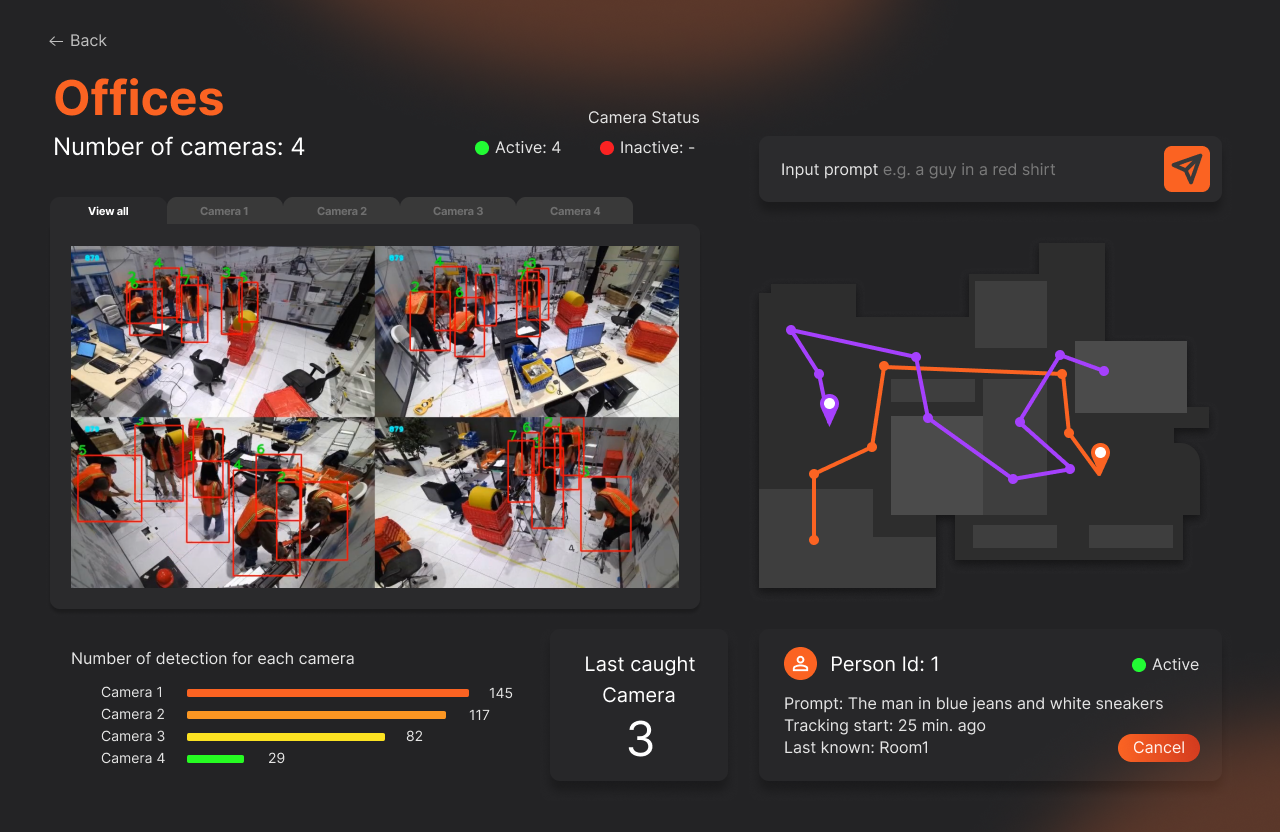
\includegraphics[width=0.8\textwidth,keepaspectratio]{jubjones/mockup/Group view.png}
    \caption{Mockup of Group View Page (Overview)}
    \label{fig:mockup-group-view}
\end{figure}

\begin{figure}[h!]
    \centering
    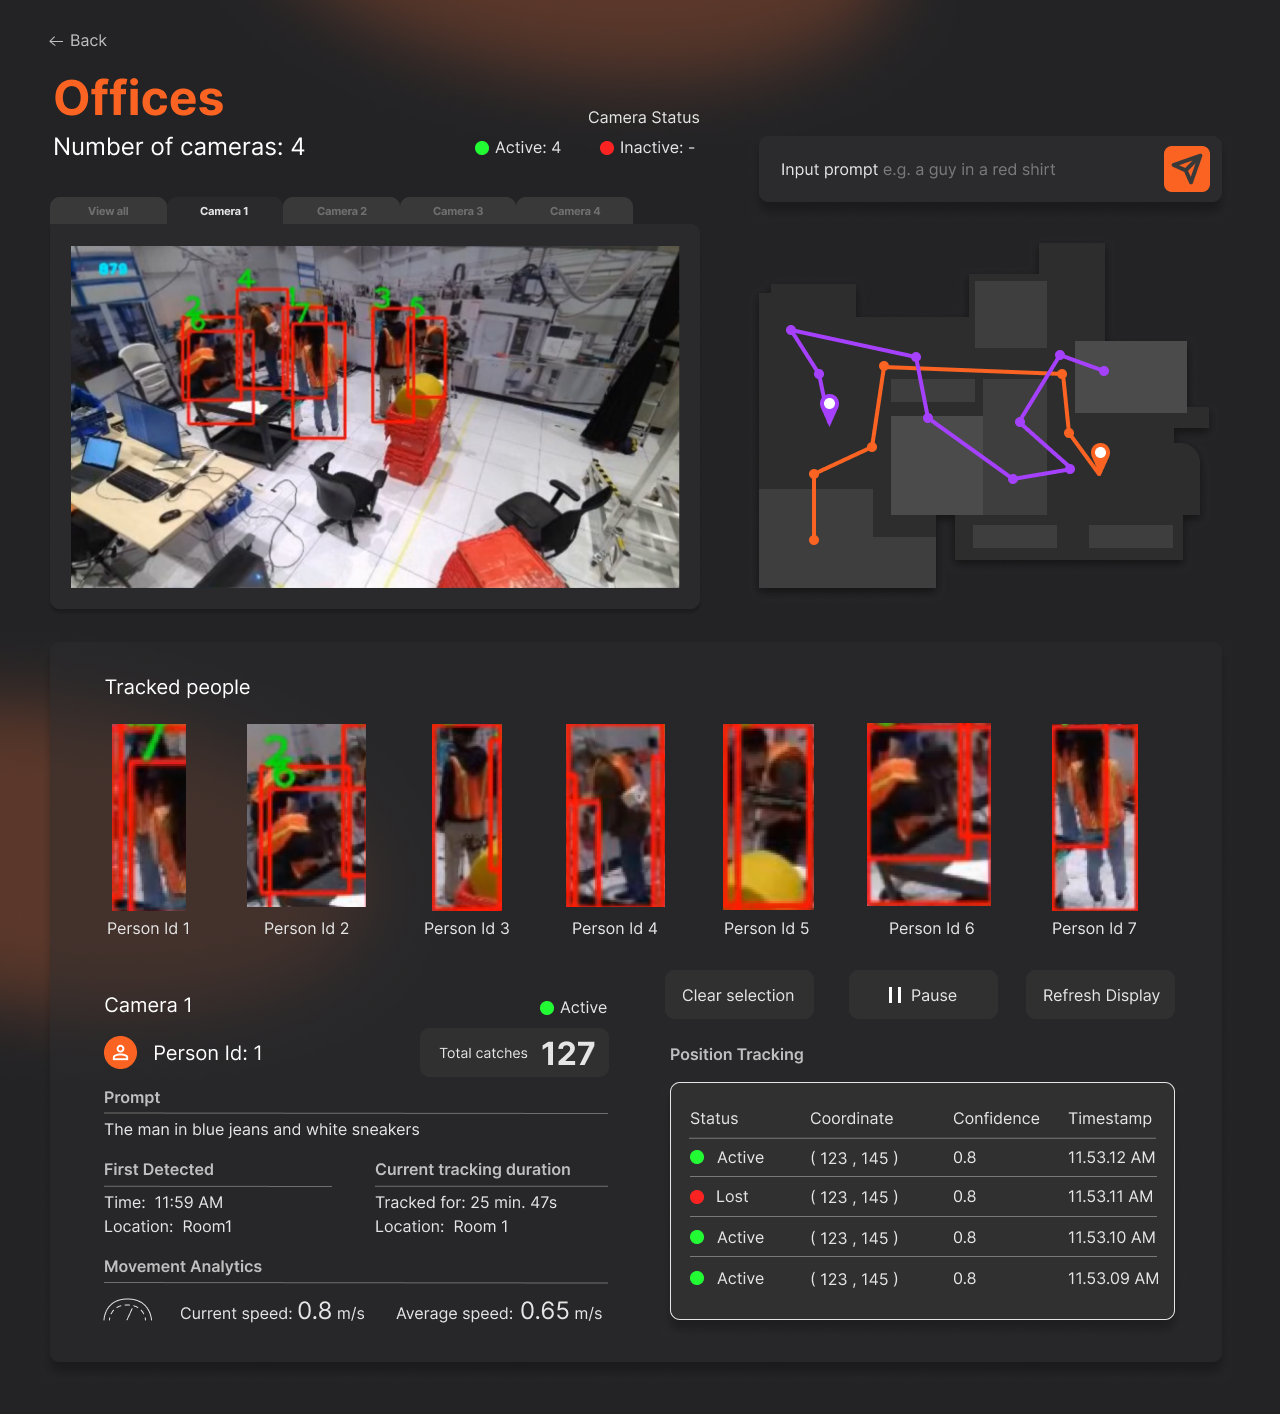
\includegraphics[width=0.8\textwidth, keepaspectratio]{jubjones/mockup/Detail view - expand.png} %Added height constraint
    \caption{Mockup of Group View Page (Expanded - Single Camera View)}
    \label{fig:mockup-group-view-expanded}
\end{figure}
\clearpage

The user interface presents an intuitive flow across multiple views as illustrated in the mockups. The Landing Page (Figure \ref{fig:mockup-landing-page}) offers users a choice between campus and factory views, followed by a date selection interface (Figure \ref{fig:mockup-landing-page-datetime}) to access specific video feed timeframes. Once a selection is made, the Group View Page (Figure \ref{fig:mockup-group-view}) displays all cameras with detected individuals, presenting a comprehensive map that visualizes tracking paths and shows detection counts per camera. This page features multiple tabs, including an overview tab showing all camera feeds simultaneously and individual tabs for specific views. For more detailed analysis, the Expanded Group View (Figure \ref{fig:mockup-group-view-expanded}) displays camera feeds with identification markers for each detected person, listing cropped images of all detected individuals below the video feed. Users can select specific individuals to focus tracking exclusively on them, viewing detailed information such as position tracking status, coordinates, confidence levels, timestamps, first detection time, current tracking duration, and movement analysis.

% Mockup End
\newpage

\section{Target and Development System}
\label{section:target-development-system} % Changed label

\subsection{Data Ingestion and Playback}
\label{subsection:data-ingestion-playback} % Added name and corrected label
% The MTMMC tracking system requires robust data handling capabilities for both ingestion and playback to support real-time person tracking across multiple cameras.

\begin{itemize}[leftmargin=80pt]
    \item \textbf{Amazon S3:} The MTMMC Dataset image files are stored in Amazon S3, providing reliable, scalable object storage. This allows for consistent access to time-stamped or sequentially named images for each camera, which is essential for synchronized playback across multiple feeds.
    \item \textbf{Frontend UI:} The user interface enables selection of specific camera views and time ranges, initiating the playback process through an intuitive and responsive control panel. This triggers backend processes to locate and retrieve the relevant image sequences.
    \item \textbf{FastAPI Backend:} Upon receiving playback requests, the backend identifies the sequence of relevant image files within the specified time range, establishes the initial playback state, and begins the core processing loop for each camera feed.
\end{itemize}

\subsection{Core Processing Pipeline}
\label{subsection:core-processing-pipeline} % Added name and corrected label
The system employs a sophisticated pipeline for processing each frame from all active camera feeds, combining object detection, tracking, and re-identification capabilities:

\begin{itemize}[leftmargin=80pt]
    \item \textbf{Faster R-CNN:} This object detection and tracking model processes each frame to identify persons and assign temporary, camera-specific track IDs. The model outputs bounding boxes, confidence scores, and tracking states for each detected individual across consecutive frames.
    \item \textbf{OSNet:} The OpenSet Network extracts appearance features (embeddings) for person re-identification. The system conditionally triggers OSNet based on specific rules including new track confirmation, track re-activation after occlusion, cross-camera handoff candidates, and periodic refreshing of long-lived tracks.
    \item \textbf{Re-Identification:} The system compares embedding vectors against a gallery of recent embeddings to associate temporary track IDs with persistent global person IDs across multiple cameras. This process utilizes both Redis for fast lookups of recently seen persons and TimescaleDB for historical embedding comparison.
    \item \textbf{Perspective Transformation:} Using pre-calculated homography matrices, the system transforms image-space coordinates to a unified top-down map coordinate system. This enables consistent tracking visualization across the entire monitored area regardless of the originating camera.
\end{itemize}

\subsection{Data Management and Communication}
\label{subsection:data-management-communication} % Added name and corrected label
To support real-time tracking and historical analysis, the system employs a combination of in-memory caching and persistent storage solutions:

\begin{itemize}[leftmargin=80pt]
    \item \textbf{Redis:} This in-memory data store caches the latest state for each active global person ID, including current map coordinates, timestamp, last camera ID, and bounding box information. Redis enables rapid lookups for real-time tracking status and visualization.
    \item \textbf{TimescaleDB:} Built as an extension to PostgreSQL and optimized for time-series data, TimescaleDB stores detailed historical tracking events with timestamps, global IDs, camera IDs, bounding boxes, and map coordinates. Vector support (pgvector) enhances embedding similarity searches for improved re-identification.
    \item \textbf{WebSocket:} FastAPI's WebSocket implementation facilitates real-time communication between the backend and frontend components. The backend pushes processed frame data including camera ID, timestamp, image URL, and tracking data with global person IDs, bounding boxes, and map coordinates.
\end{itemize}

\subsection{Frontend Implementation}
\label{subsection:frontend-implementation} % Added name and corrected label
The user interface provides intuitive visualization and interaction capabilities to monitor tracked individuals across multiple camera views:

\begin{itemize}[leftmargin=80pt]
    \item \textbf{React:} This JavaScript library forms the foundation of the user interface components, providing a responsive and component-based architecture that efficiently updates based on state changes.
    \item \textbf{Zustand:} This lightweight state management solution stores and manages tracking data received via WebSocket, organizing it by camera ID, global person ID, and timestamp for efficient rendering and interaction.
    \item \textbf{Leaflet.js:} This interactive mapping library visualizes the top-down perspective of tracked individuals, displaying their real-time positions and movement paths on a shared coordinate system derived from the homography transformations.
    \item \textbf{Canvas/SVG:} These rendering technologies are used to overlay bounding boxes and labels on camera feed images, providing visual identification of tracked individuals within each view.
\end{itemize}

\subsection{Deployment Infrastructure}
\label{subsection:deployment-infrastructure} % Added name and corrected label
The system is designed for containerized deployment with comprehensive monitoring capabilities:

\begin{itemize}[leftmargin=80pt]
    \item \textbf{Docker:} All system components are containerized for consistent deployment across environments, with the backend requiring GPU access for efficient execution of deep learning models.
    \item \textbf{Nginx:} Serving as the entry point and reverse proxy, Nginx handles HTTPS termination, request routing, WebSocket proxying, and potential load balancing for scaled backend instances.
    \item \textbf{Kubernetes:} This container orchestration platform manages, scales, and ensures the reliability of all system services in production environments, with Docker Compose available for simpler development setups.
    \item \textbf{Prometheus \& Grafana:} This monitoring stack collects and visualizes system metrics including CPU, RAM, and GPU utilization, while Loki and Promtail handle log aggregation and collection for comprehensive system observability.
\end{itemize}

\subsection{MLOps Workflow}
\label{subsection:mlops-workflow} % Added name and corrected label
The machine learning operations workflow supports model development, training, and deployment:

\begin{itemize}[leftmargin=80pt]
    \item \textbf{MLflow:} This platform provides experiment tracking capabilities for logging parameters, metrics, and artifacts during model development, along with a model registry for versioning and staging trained models.
    \item \textbf{Dagshub:} Complementing MLflow, this service enhances collaboration on machine learning projects with extended versioning and sharing capabilities for models and datasets.
    \item \textbf{CI/CD Pipeline:} The system supports continuous integration and deployment for model updates, fetching approved model artifacts from the registry, building new Docker images, and updating running services with minimal downtime.
\end{itemize}